\chapter{Aplicación Android}

Para este proyecto se ha elegido la plataforma Android como interfaz gráfica ya que es la más utilizada en dispositivos móviles y es en éstos donde el desarrollo podría tener un mayor uso.
Al igual que se consulta en el móvil el tiempo que se tardará en ir de un punto a otro, se podría consultar la seguridad de la ruta que vamos a realizar en bicicleta para evaluar el riesgo y replantearse el medio de transporte que se utilizará.
Siendo la aplicación Google Maps la más utilizada como GPS, en este proyecto se ha consultado la ruta a través de la API Directions de Google\cite{apiDirections}, la cual proporcionará previsiblemente la misma ruta que posteriormente el usuario seguirá por GPS hasta su destino.

Para el desarrollo se ha priorizado mostrar las características de la ruta y no tanto el aspecto visual ni la eficiencia. En una aplicación desarrollada para un uso cotidiano lo ideal sería mostrar pocos datos sobre los datos sobre la ruta, marcar el valor numérico asociado a ella y mencionar las vías con más peligro para que se mantenga más atención. Sin embargo, para este proyecto se ha preferido mostrar el máximo número de datos obtenidos (como el número de accidentes de cada tipo) y se ha priorizado la visualización por parte del usuario de los mismos. Dado que el cálculo de la peligrosidad no ha seguido ningún patrón ni regla, únicamente una aproximación de la importancia que se le podría dar a cada elemento, se ha optado por esto para que quien desee valore subjetivamente los datos dispuestos.

Todo el código de la aplicación Android se encuentra en el repositorio de Github \cite{githubRepositorio} en la ruta \url{ProyectoAndroid/app}.

Durante la ejecución de la aplicación se pueden distinguir dos fases bien diferenciadas: la obtención de la ruta y el cálculo de ella.









\clearpage
\section{Obtención de la ruta}
La ruta como ya se ha mencionado anteriormente es obtenida a partir de API Directions de Google. En dicha ruta no es posible conocer el nombre de las calles ni su identificador ya que se obtienen una serie de coordenadas por las que el navegador guía al usuario.
El fin de este proyecto es conocer la seguridad de cada una de las calles, por lo tanto se deben obtener las vías en las que se encuentran esos puntos. Para ello se ha creado una base de datos en SQLite dentro de la propia aplicación para hacer la búsqueda de esas coordenadas y así poder realizar las demás consultas.


\subsection{Creación BBDD coordenadas}
Como se ha mencionado anteriormente, el primer paso para obtener las calles transitadas es crear la base de datos con las coordenadas para posteriormente consultar en ella la ruta.
Las coordenadas son proporcionadas por el Ayuntamiento de Madrid y se encuentran, como los anteriores datasets, en el portal de datos.madrid y en formato CSV \cite{coordenadas_DatosMadrid}.
Dicho dataset contiene numerosos errores en sus coordenadas representadas en grados. Se puede comprobar como una misma calle está representada con puntos opuestos de la ciudad. Esto implicaría que la ruta que se obtuviese con esos datos representase valores irreales y mostrase un gran número de calles que nada tendrían que ver con el recorrido. Dado que los puntos proporcionados por Google están separados por pocos metros y que la gran mayoría de calles están representadas por más de 5 coordenadas, este error produciría que el resultado final fuese completamente diferente al esperado.
Tras varias pruebas se ha detectado que las coordenadas representadas en UTM si son correctas, por lo tanto se han utilizado estas últimas. Para su uso, dado que los puntos proporcionados por la API de Google son en formato decimal, se han transformado a este formato. Para ello se ha hecho uso de un código obtenido de la siguiente url: \url{https://stackoverflow.com/questions/343865/how-to-convert-from-utm-to-latlng-in-python-or-javascript/344083#344083} con ligeras modificaciones. El cuadrante para España necesario para esta transformación es 30 y ha sido obtenido de la web de la Junta de Andalucía \cite{UTM_cuadrante_andalucia}.

En un primer momento se tomó la decisión de dividir en cuadrantes el territorio para poder realizar una búsqueda más rápida. Al utilizarse SQL el proceso de búsqueda ya está optimizado y en este caso se ha comprobado que es menos eficiente este método, por lo tanto se ha descartado. Es posible que para ciudades más grandes si sea interesante dicho filtro y es por ello que se ha conservado el código para realizarlo. Sin embargo, para el proyecto actual se ha omitido esta transformación.

El código al que se hace referencia en esta sección se encuentra en el repositorio de Github 	\cite{githubRepositorio} en la ruta \url{ProyectoPython/tratamientoDataCoordenadas.py}.
En dicho fichero se encuentran las funciones ``utmToLatLng`` (encargada de transformar las coordenadas UTM  a decimal) y ``calcularCoordenadasDecimales`` (encargada de transformar las coordenadas en grados, minutos y segundos a decimal). El resto de las funciones que contiene son tienen como finalidad asignar los cuadrantes (opción finalmente descartada en este proyecto), transformar el dataset de coordenadas con los nuevos valores decimales y generar los ficheros necesarios para añadir los datos a la aplicación Android.

Para crear la base de datos en Android se ha generado en primer lugar una tabla con los campos ID$\_$VIA, COD$\_$POSTAL, LATITUD, LONGITUD y codCuadrante. No todos los campos están siendo usados en esta práctica, aunque si se ha decidido conservarlos por si en un futuro fuesen necesarios. Actualmente se insertan únicamente el identificador de vía, la latitud y la longitud. A los campos no requeridos se insertan valores vacíos.
La primera vez que se inicia la aplicación se cargan los aproximadamente 100.000 registros de coordenadas que hay en Madrid con sus identificadores de calles. Este proceso tarda unos 10 segundos, aunque puede variar entre dispositivos y solo se realiza una vez a no ser que se desinstale o se borren los datos.

Crear una base de datos con las coordenadas permite que el móvil sea mucho más rápido a la hora de realizar consultas sobre la ruta ya que no requiere conectarse a una API y al ser un gran número de consultas por ruta posibilita que se genere a una mayor velocidad.

Dicho código se puede encontrar en Todo el repositorio de Github \cite{githubRepositorio} en la ruta \url{ProyectoAndroid/app/src/main/java/com/example/androidrutasbicimadrid}.















\clearpage
\subsection{Conexión API Google Directions y lista de calles transitadas}
En esta sección se va a tratar tanto la conexión y obtención de los puntos de la ruta, como de su búsqueda en la base de datos para así recibir la lista de calles transitadas en la misma.

De nuevo el código relativo a esta sección se encuentra en el repositorio de Github \cite{githubRepositorio} en la ruta \url{ProyectoAndroid/app/src/main/java/com/example/androidrutasbicimadrid}.

En primer lugar, se le pide al usuario la dirección de origen y destino. Una vez insertados se genera una url para la API con dicha información y con la clave para su uso. La información relativa al uso de la API se encuentra en la web de Google \cite{apiDirections}. Para insertar los valores de origen y destino se separan los componentes con ``+`` y se le añade a cada uno ``,Madrid`` ya que siempre van a ser en el ámbito de esta ciudad y de esta forma se evita que se generen rutas inválidas por nombres iguales en distintas partes del mundo. Finalmente se añade ``$\&$avoid=highway$\&$mode=bicycling``. Esto nos permite obtener la ruta que nos proporcionaría el navegador en modo bicicleta y evitando autopistas (ya que las bicicletas tienen prohibida su entrada en estas).


\begin{figure}[h]
	\centering
	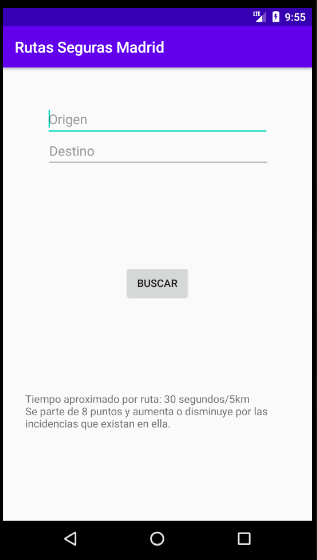
\includegraphics[angle=0, width=0.3\textwidth]{images/android/camposRuta.png}  
	
	\caption{Pagina Inicio Aplicación}
	\label{fig:diagramaOntologAccid}
\end{figure}


Cabe destacar que la clave que se está utilizando en este proyecto para la API de Google será restringida o cancelada un tiempo después de la finalización del proyecto. Debido a que no se va a comercializar y cualquiera podría reutilizar el código, se tendría que modificar dicho campo para utilizar una clave propia. Para que pueda mostrarse correctamente y probarse se ha decidido compartir durante cierto, aunque pasado un plazo se cancelará para evitar un mal uso de la misma.




Una vez se ha hecho la petición http se obtiene un fichero JSON con las características de la ruta. Para su tratamiento se han tenido de nuevo en cuenta las especificaciones y ejemplos proporcionados por en la web de Google \cite{apiDirections}.
De este fichero se obtienen los valores distancia y duración y todas y cada una de las coordenadas de la ruta. Para ello se ha creado una clase ``Coordinate`` cuyas propiedades son longitud y latitud. Para obtenerlas se recorre los distintos ``steps`` de los que está compuesto el JSON y se listan. El código detallado se encuentra en la ruta antes mencionada en el fichero MainActivity.java, en la función llamada getArrayCoordenadas.






Tras tener dicha lista de coordenadas, han de buscarse en la base de datos antes generada para obtener los identificadores de las vías por las que transcurre. Para ello se realizan peticiones SQL  a la base de datos con cada iteración de la lista anterior.
Al ser la ruta un conjunto de coordenadas separadas entre si por varios metros de distancia, es muy improbable que coincida exactamente con el punto almacenado (que sigue el mismo procedimiento). Es por ello que a la hora de buscar los puntos se ha aplicado un margen de error en varias fases. La primera de ellas de 15 metros, la segunda de 30, la tercera de 60... De modo que aun no siendo el punto exacto se pueda encontrar el más cercano a esa posición.
Al aplicar este margen de error podría darse el caso de que para un mismo punto existan varias calles sin ser necesariamente un cruce, en un radio de 15 metros puede haber varias coordenadas. Se genera por cada punto una lista de calles ``posibles`` y una lista de diferencias. Estas se calcularán con la suma del valor absoluto de las diferencias entre sus latitudes y longitudes (las de la coordenada de la ruta y la de la base de datos). Una vez se tengan estas listas, a ese punto le corresponderá la de menor diferencia, es decir, la más próxima.
El código detallado se encuentra en la ruta antes mencionada en el fichero PeticionesBBDD.java, en la función llamada getListaCallesPosibles.

Una vez finalizado este proceso para todas las coordenadas se tendrá una lista de calles, a la cual se le eliminarán los duplicados y de esta forma se podrá consultar las incidencias de las calles por las que la ruta transcurre.















\clearpage
\section{Cálculo de Seguridad de ruta}

Para el cálculo de la ``seguridad`` de la ruta, como se ha explicado anteriormente, no se ha seguido ninguna regla ni ningún procedimiento estadístico. Es por ello que no se consideran fiables las operaciones realizadas.
Sin embargo, si ha querido mostrarse la utilidad de los datos enlazados para una aplicación como esta y ha querido realizarse una aproximación ``subjetiva`` acorde a los datos existentes.

Para el cálculo se tendrán en cuenta los ciclocarriles, calles tranquilas y accidentes. A cada uno se le asignará un valor proporcional sobre la importancia que tienen en la ruta (3 para ciclocarriles, 2 para calles tranquilas y 5 para accidentes). En cada calle transitada se comprobará si tiene o no ciclocarril y si es ``calle tranquila``. En caso de serlo se sumará el modificador anterior dividido por el número de calles (de esta forma por ejemplo si todas las vías de la ruta son tranquilas, se sumarán al cálculo 2 puntos).
Para accidentes se han tenido en cuenta más variables como son la lesividad y el tipo de persona afectada. Primero se calculará la gravedad del siniestro (10 en caso de fallecimiento, 5 accidente grave y 1 leve), y posteriormente se multiplicará este valor por la ``importancia que le da el conductor de la bicicleta``. Esto último no es del todo correcto, pero se ha considerado que la persona que desea valorar la seguridad de la ruta da más importancia a su integridad (las bicicletas están más desprotegidas) que a la de otro conductor. Siguiendo esta línea se ha multiplicado la gravedad por 3 en caso de ser el conductor el afectado, por 2 en caso de ser un peatón o viajero, y por 1 en caso de ser otros.
Para el caso de accidentes se ha usado el mismo método que los anteriores con el modificador y la gravedad del accidente, aunque con ligeras modificaciones. Se ha puesto un valor tope (2 puntos) por calle, ya que vías con mucha longitud y muy peligrosas podrían reducir incluso los 10 puntos máximos que puede tener la ruta, por tanto debe restringirse.

Por último, es importante destacar que se parte de 8 puntos, es decir, que a partir de ahí se sumará o restará dependiendo de las incidencias detectadas. Se ha elegido esta cantidad inicial ya que permitía cierto margen para que las rutas pudiesen llegar a 10 en caso de haber muy pocos accidentes y que en zonas muy transcurridas no rozase constantemente el 0.

El código detallado se encuentra en la ruta antes mencionada en el fichero MainActivity.java, en la función llamada getNotaRuta y getGravedadAccidente.

Para obtener los datos necesarios para este proceso se ha hecho uso de Jena y de las consultas explicadas en el capítulo anterior. Dicho se encuentra en el fichero JenaRequest.java y contiene funciones con los valores de retorno antes mencionados.

Como se mencionó anteriormente se ha dado prioridad a mostrar las características de la ruta en vez de a únicamente el cálculo. Es por ello que en este proceso se ha detallado la puntuación que se ha sumado y restado por cada incidencia. De este modo cualquiera que lo use podría calcular la nota acorde a sus criterios.


En los siguientes ejemplos se observa cómo se han mostrado la nota y las incidencias de la ruta en la aplicación final desarrollada.


\clearpage
\begin{figure}[h]
	\centering
	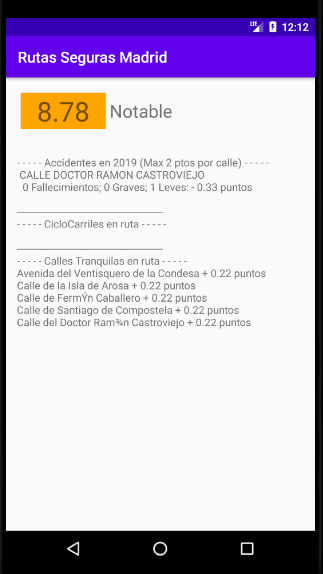
\includegraphics[angle=0, width=0.3\textwidth]{images/android/captura2.png}  
	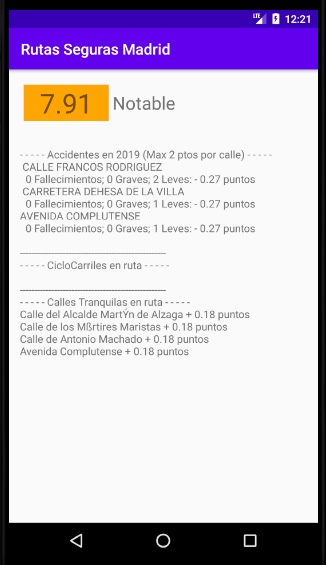
\includegraphics[angle=0, width=0.3\textwidth]{images/android/captura4.png} 
	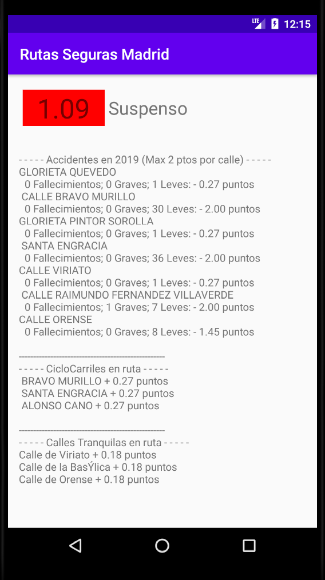
\includegraphics[angle=0, width=0.3\textwidth]{images/android/captura3.png}  
	
	\caption{Ejemplos de rutas}
	\label{fig:diagramaOntologAccid}
\end{figure}

En las capturas anteriores se muestran 3 rutas diferentes consultadas en Madrid.
La primera corresponde a la ruta entre Metro Mirasierra y Metro Peñagrande. Como se puede observa es bastante segura aun no teniendo ciclocarriles. Pocos accidentes han ocurrido en las calles por las que se transita y se han catalogado varias de ellas como tranquilas.
Lo mismo ocurre en la segunda captura, ruta entre Metro Valdezarza y E.T.S Agrónomos (Ciudad universitaria). En ésta han ocurrido unos pocos más accidentes leves, pero sigue considerándose segura.
Sin embargo, en la tercera imagen se muestra la ruta entre Bravo Murillo 1 y Calle de Orense 5. Se puede observar que hay ciclocarriles que aumentan en cierta medida la seguridad, sin embargo al ser una zona céntrica y con calles estrechas y muy concurridas, han ocurrido muchos accidentes, algunos de ellos graves, que han reducido drásticamente la seguridad de la misma. Cabe destacar en esta que la calle Raimundo Fernández Villaverde ha restado 2 puntos al cómputo general (que es el máximo permitido por calle).


